\documentclass[
	11pt
]{beamer}

\graphicspath{{img/}} % Specifies where to look for included images (trailing slash required)

\usetheme{Boadilla}
\usepackage{booktabs} % Allows the use of \toprule, \midrule and \bottomrule for better rules in tables
\usepackage{amsmath}
\usepackage[T1,TS1,T2A]{fontenc}
\usepackage[utf8]{inputenc}
\usepackage[english,russian]{babel}



\title[Анализ в сфере образования]{Изучение группового обучения в общем образовании} 
\author[Машалов Никита]{Машалов Никита} 

\begin{document}
\DeclareFontShape{OT1}{cmss}{b}{n}{<->ssub * cmss/bx/n}{} 

\begin{frame}
    \begin{figure}
        
\includegraphics[width=0.2\linewidth]{assets/MIPT.png}
    \end{figure}
    \titlepage % Output the title slide, automatically created using the text entered in the PRESENTATION INFORMATION block above
\end{frame}

\begin{frame}
    \frametitle{План презентации} % Slide title, remove this command for no title
    \tableofcontents
\end{frame}


Образование несет важную роль в экономике стран пост-индустриального развития.

В разделе описаны подходы к модельному исследованию командной деятельности.

Аналитическое изучение кооперативной деятельности выполняется в теории совместных игр 
В этом случае результирующий вклад задается агрегирующий усилия игроков функцией.
$$
 f_i(s) = \tilde{f_i} \left(s_i, \sum_{j=1}^n s_j \right),
$$

Классическим примером производственной функции является функция Кобба Дугласа

$$
    Q = A L^\beta K^\alpha,
$$
где \begin{itemize}
    \item $Q$ - общий объем производства;
    \item $L$ - вложенный труд; 
    \item $K$ - денежный капитал;
    \item $A$ - мультипликатор производства;
    \item $\alpha$ и $\beta$ - параметры эластичности выпуска.
\end{itemize}


Постоянная эластичность замещения обобщает функцию 
Кобба-Дугласа \cite{mcfadden1963constant}:
$$
    Q = A (a \cdot K^p + (1-a)\cdot L^p)^{\frac{v}{p}},
$$
где \begin{itemize}
    \item $\rho$ - параметр замещения; 
    \item $\alpha$ и $\beta$ - параметры эластичности выпуска.
\end{itemize}

При $\rho \rightarrow 0$ функция вырождается в функцию Кобба-Дугласа.

Случай многих аргументов запишется как:
$$
    Q \sum_i \left(\alpha_i x_i^\rho \right)^{\frac{\beta}{\rho}}, \sum_i \alpha_i=1
$$





\subsection{Мотивация работы}

\begin{frame}
    \frametitle{Постановка магистерской работы}
    \centering
    \begin{itemize}
        \item Сложность задания $d$, знания учащегося $u$
        \item Модель Эло $$
            p(x=1|d,u) = \frac{1}{1+\exp(d-u)}
        $$
        \item Адаптивные алгоритмы задают оптимальный уровень попыток $s^*$ на
        исход выполнения задания 
    \end{itemize}
    \begin{block}{Алгоритм Роббинса-Монро}
        Пускай $x$ - бернулевская случайная величина с параметром $s=f(d)$, где $f(x)$ - выпуклая.
        Тогда для cхема пересчета $d_t=\mathbf{x}_t + a_t (s^* - x_t)$ с шагами $a_t$ удовлетворяющих условиям
        $\sum_{t=0}^{\infty} a_t = \infty, \sum_{t=0}^{\infty} a_t^2 < \infty$,
        выполняет cпуск к целевому значению $\lim_{t \rightarrow \infty} d_t = d^*$, где $d^* : s(d^*) = s^*$.
    \end{block}
\end{frame}



\begin{frame}
  \centering \Large
  \emph{Постановка для диссертации}
\end{frame}


\begin{frame}
    \frametitle{Индивидуальное обучение}
    \centering

    \begin{figure}
        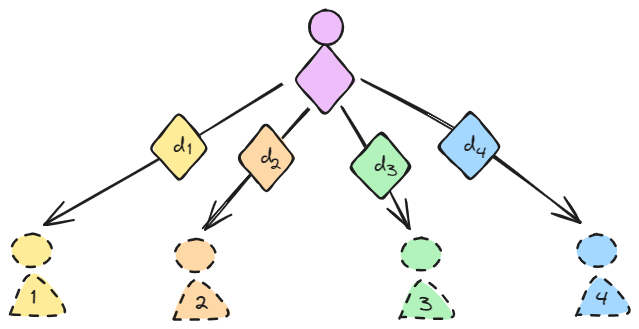
\includegraphics[width=0.9\linewidth]{assets/setting/ideal.excalidraw.png}
    \end{figure} 
\end{frame}

\begin{frame}
    \begin{block}{Постановка}
        Каждый учащийся $i$ получает задачу сложности $d_i$, соответствующую текущему развитию
    \end{block}

    \begin{exampleblock}{Преимущества}
        \begin{itemize}
            \item адаптивное обучение
            \item сроки исполнения выбираются из потребностей обучающегося
        \end{itemize}

    \end{exampleblock}

    \begin{alertblock}{Недостатки}
        \begin{itemize}
            \item проверка большого числа заданий
            \item координация работы
        \end{itemize}
    \end{alertblock}
\end{frame}


\begin{frame}
    \frametitle{Коллективное обучение}
    \centering
    \begin{figure}
        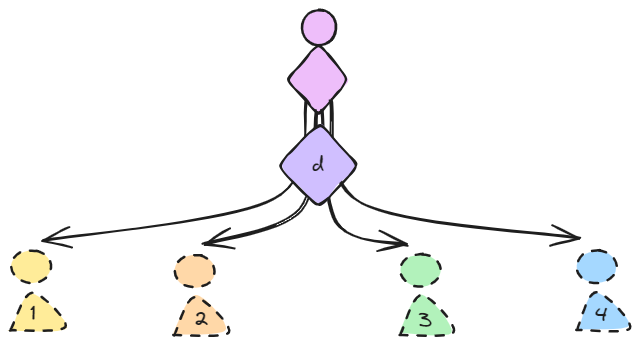
\includegraphics[width=0.9\linewidth]{assets/setting/real.excalidraw.png}
    \end{figure} 
\end{frame}

\begin{frame}
    \begin{block}{Постановка}
        Все обучающиеся выполняют одну задачу сложности $d$
    \end{block}
    \begin{exampleblock}{Преимущества}
        \begin{itemize}
            \item возможность предварительной подготовки программы
            \item поощряет соревновательный дух
            \item относительная простота проверки
        \end{itemize}
    \end{exampleblock}
    \begin{alertblock}{Проблемы}
        \begin{itemize}
            \item отсутствие интереса у отстающих и одаренных обучающихся
            \item сложность учета индивидуальных потребностей
        \end{itemize}
    \end{alertblock}
\end{frame}


\begin{frame}
    \frametitle{Постановка для кандидатской диссертации}
    \centering
    \begin{block}{Цель}
        Определение оптимальных стратегий обучений в группах с использованием адаптивных алгоритмов сложности
    \end{block}

    \begin{block}{Задачи}
        \begin{itemize}
            \item демонстрация несостоятельности базового алгоритма Роббинса-Монро для коллективного обучения
            \item изучение распределения нагрузки между учащимися с учетом супераддитивности функций совместной работы
            \item разработка алгоритма адаптивной сложности для работы с группами
        \end{itemize}
    \end{block}

\end{frame}


\section{Теория}

\begin{frame}
    \frametitle{Совместные задания для групп}
    \centering
    \begin{figure}
        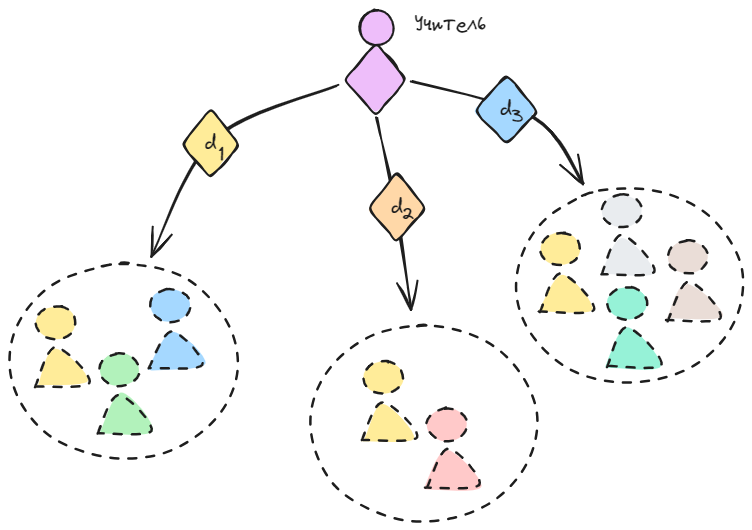
\includegraphics[width=0.8\linewidth]{assets/setting/groups.excalidraw.png}
    \end{figure}
\end{frame}

\begin{frame}
    \frametitle{Описание}
    \begin{block}{Постановка}
        Учащиеся объединяются в $k$ групп. Каждой группе $i$ предлагается задача сложности $d_i$. 
    \end{block}

    \begin{exampleblock}{Преимущества}
        \begin{itemize}
            \item оптимальное число заданий к проверке
            \item обучение командной работе
            \item \textbf{применимость адаптивного обучения} 
        \end{itemize}
    \end{exampleblock}

    \begin{alertblock}{Проблемы}
        \begin{itemize}
            \item неравномерное распределение нагрузки в группе
            \item неясность в выборе сложности задания
        \end{itemize}
    \end{alertblock}
\end{frame}

\begin{frame}
    \frametitle{Алгоритм Роббинса-Монро для функций многих переменных}
    Обобщение алгоритма для случая многомерной функции отклика 
    задаёт условия на параметры схемы. \footnote{Xiong, Cui, and Jin Xu. "Efficient Robbins–Monro procedure for multivariate binary data."}
    \begin{block}{Алгоритм Роббинса-Монро для случая многих переменных}
        Пусть $\vec{x}$ - вектор бернулевских случайных величин с параметрами $\vec{s}=f(\vec{d})$, где $f(\vec{x})$ - выпуклая.
        Тогда cхема пересчета $d_t=\vec{x}_t + A^{(t)} (s - \vec{x}_t)$ с шагами $A^{(t)}$ удовлетворяющих условиям:
        $\forall t,j \rightarrow a_{jj}^{(t)} >0,
        \sum^{\infty}_{t=1} a_{jj}^{(t)} = \infty,
         \sum_{n=1}^\infty (a^{(t)}_{jj})^2 < \infty$
        сходится по вероятности к целевому значению $\vec{s}^*$
    \end{block}
\end{frame}


\begin{frame}
    \frametitle{Супераддитивность в групповом образовании}
    \begin{block}{Эффективность совместногого обучения}
        Считаем, что эффективность учащихся задается как гауссова случайная величина$$
            \vec{x} \sim \mathcal{N}(\vec{\mu}, \Sigma).
        $$
        Матрица ковариации $\Sigma$ задает эффективность командной работы
    \end{block}
    \begin{block}{Супераддитивность}
        Супераддитивной называется функция $f$ для которой
        \begin{equation}
            \forall x, y, x+y \in \text{dom}(f) \rightarrow f(x+y) \ge f(x) +f(y) 
        \end{equation}
    \end{block}

    \begin{block}{Функции к изучению}
        \begin{itemize}
            \item min-sum $\sum_{i} min([\vec{x}]_i,s^*)$, гдe $s^*$ - порог отсечки
            \item max-mean $N \cdot \bar{x} + \max_i(\vec{x} - \bar{x})$
            \item квадратичная форма $\vec{x}^T A \vec{x}$
        \end{itemize}
    \end{block}
\end{frame}
% \subsection{Обобщение}

\begin{frame}
    \frametitle{Обобщение}
    \begin{figure}
        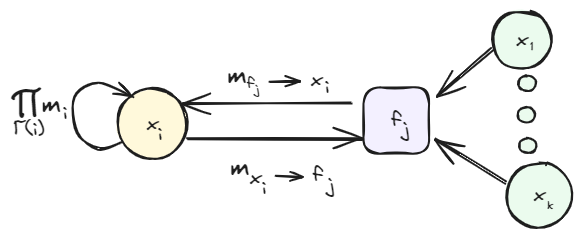
\includegraphics[width=0.8\linewidth]{assets/message_passing.excalidraw.png}
    \end{figure}
    $$
        \begin{aligned}
            &m_{f_j \rightarrow x_i} = \sum_{X_j \backslash x_i} f_j(X_j) \prod_{k\in N(j) \ i} m_{x_k \rightarrow f_j}\\
            &m_{x_i \rightarrow f_j} = \prod_{s \in N(i) \backslash j} m_{f_s \rightarrow x_i}
        \end{aligned}
    $$
\end{frame}











Образование несет важную роль в экономике стран пост-индустриального развития.

В разделе описаны подходы к модельному исследованию командной деятельности.

Аналитическое изучение кооперативной деятельности выполняется в теории совместных игр 
В этом случае результирующий вклад задается агрегирующий усилия игроков функцией.
$$
 f_i(s) = \tilde{f_i} \left(s_i, \sum_{j=1}^n s_j \right),
$$

Классическим примером производственной функции является функция Кобба Дугласа

$$
    Q = A L^\beta K^\alpha,
$$
где \begin{itemize}
    \item $Q$ - общий объем производства;
    \item $L$ - вложенный труд; 
    \item $K$ - денежный капитал;
    \item $A$ - мультипликатор производства;
    \item $\alpha$ и $\beta$ - параметры эластичности выпуска.
\end{itemize}


Постоянная эластичность замещения обобщает функцию 
Кобба-Дугласа \cite{mcfadden1963constant}:
$$
    Q = A (a \cdot K^p + (1-a)\cdot L^p)^{\frac{v}{p}},
$$
где \begin{itemize}
    \item $\rho$ - параметр замещения; 
    \item $\alpha$ и $\beta$ - параметры эластичности выпуска.
\end{itemize}

При $\rho \rightarrow 0$ функция вырождается в функцию Кобба-Дугласа.

Случай многих аргументов запишется как:
$$
    Q \sum_i \left(\alpha_i x_i^\rho \right)^{\frac{\beta}{\rho}}, \sum_i \alpha_i=1
$$






\subsection{Вектор Шепли}

Базовой кооперативной игрой являются координационные.
Супераддитивной называется функция $f$ для которой
\begin{equation}
    \forall x, y, x+y \in \text{dom}(f) \rightarrow f(x+y) \ge f(x) +f(y) 
\end{equation}


Свойства:
\begin{itemize}
    \item Эффективность $\phi_A(v) + \sum_{i \in N} \phi_i(v) = v_a(N)$
    \item Симметричность относительно типа $\forall i,j \in N \rightarrow \phi_i(v) = \phi_j(v)$
    \item Линейность 
\end{itemize}

\subsection{Вектор Шепли}


\subsection{Рассмотрение в приближение среднего поля}
\section{Заключение}
\begin{frame}
    \frametitle{Заключение}
    
    \begin{itemize}
        \item тема диссертационной работы
        \item изучаются постановки командных заданий для случая супераддитивных функций
        \item заданные постановки изучаются с целью выработки оптимального алгоритма задания сложности
        \item 2 статьи готовы к публикации
    \end{itemize}
\end{frame}


\begin{frame}
    \centering \Large
  \emph{Cпасибо за внимание!}
\end{frame}

\end{document}




